%% Paper 2: the learning potential of small language models for tool use (E13 to E19).
%% Target: Knowledge-Based Systems (Elsevier), on Elsevier's CAS template (cas-dc, two columns), which the KBS Guide for
%% Authors links; double-column layout is permitted for LaTeX submissions.
%% Build: tectonic main.tex   (thumbnails/: the small icons the template prints beside the email address)
%% Status: design and setup outlined in full; results, analysis and discussion left until E19 is complete.
%% Grey bullets are notes for the writing, not text; details come from lab/e13..e19/notes.md and the code.
%% KBS Guide for Authors (checked 21 Nov 2026): research papers preferably <= 20 double-spaced pages including tables
%% and figures (a soft limit); abstract <= 250 words; 1-7 keywords; 3-5 highlights of <= 85 characters, submitted as a
%% separate file (highlights.txt); numbered references in square brackets, in order of appearance; figures also
%% uploaded as separate files; research data deposited in a repository (Option C).
%% Page target in this layout: about 12-15 pages, references included.
\documentclass[a4paper,fleqn]{cas-dc}

\usepackage{amssymb,amsmath}
\usepackage[numbers,sort&compress]{natbib}
\usepackage{booktabs}
\usepackage{multirow}
\usepackage{graphicx}
\usepackage{xcolor}
\usepackage{enumitem}
\usepackage{tikz}
\usepackage{xurl}  % long URLs (references, data availability) break at any character
\usetikzlibrary{positioning,arrows.meta}
\hypersetup{hidelinks}

% outline notes: shown in grey while drafting; replace each with prose
\newenvironment{outline}{\color{gray}\begin{itemize}[leftmargin=1.5em,itemsep=1pt,topsep=3pt]\small}{\end{itemize}}
\newcommand{\todo}[1]{\textcolor{red!70!black}{[TODO: #1]}}

\begin{document}

\shorttitle{Learning potential of small language models}
\shortauthors{S. Kongsilp}
\title [mode = title]{How Much Can Small Language Models Learn on the Job?\\
Measuring the Learning Potential of Notes, Retrieval and LoRA for Tool Use}
\author[1,2]{Sirisilp Kongsilp}[]
\cormark[1]
\ead{sirisilp.k@ku.th}
\ead{tai@kratai.com}
\affiliation[1]{organization={Department of Computer Engineering, Faculty of Engineering, Kasetsart University},
  addressline={50 Ngamwongwan Road, Chatuchak}, city={Bangkok}, postcode={10900}, country={Thailand}}
\affiliation[2]{organization={Decentralized Science, Inc.},
  addressline={2261 Market Street, STE 22858}, city={San Francisco}, state={CA}, postcode={94114}, country={USA}}
\cortext[1]{Corresponding author}
\begin{abstract}
Small language models (0.8B--1.7B nominal parameters) increasingly run on devices and must use tools they were
not trained for. We build an evaluation protocol for learning on the job and use it to measure the \emph{learning
potential} of six models from five families: the most a model gains when feedback is perfect. Each works through the
same 1,200 multi-turn tool-use tasks, built on the Berkeley Function Calling Leaderboard's (BFCL) tools but never its
questions, learning by one of three on-device methods: self-written notes, retrieved worked examples, or
continual low-rank adaptation (LoRA). An oracle gives the expected calls (teaching) or only pass or fail
(judging). We test learning on 200 unseen tasks every 100 tasks and on the BFCL v4, with key runs over
three seeds; tasks, code and per-question results are released. Models that cannot make a valid multi-turn call (below the floor) gain at most a point from notes or
worked examples, yet LoRA lifts two of them by about ten points on BFCL; notes help no model's multi-turn score. Learning has
side effects: trained on expert tool calls, every model learned to call tools when none fits, and a reasoning
model was harmed by expert targets but not by its own verified successes. Above the floor, gains shrink on
BFCL to a few points, below what its 200 target questions resolve. Teaching is needed to pass the floor; beyond it,
learning from one's own successes gained no less than teaching on BFCL and spared the reasoning model.
\end{abstract}
\begin{keywords}
small language models \sep tool use \sep function calling \sep continual learning \sep LoRA \sep
retrieval-augmented generation \sep in-context learning
\end{keywords}
\maketitle

%% ---------------------------------------------------------------------------------------------------------------
\section{Introduction}\label{sec:intro}
Small language models of about one billion parameters now run on phones and laptops, where they keep data private and
respond without a network \citep{wang2025comprehensive}. Increasingly they are asked to act through tools: to call
functions and APIs, often over several turns of a conversation \citep{patil2025berkeley}. Tool use is where such a model
most often meets something new, a tool or a way of combining tools that its training did not cover. Sending its data
back for retraining is often not an option, so the model would have to learn \emph{on the job}, from the tasks it does.

How much can a model of this size learn from practice, and by which route? It can learn through its context, by
writing notes about what worked \citep{suzgun2026dynamic,zhang2026agentic} or by retrieving past trajectories as worked
examples \citep{zheng2024synapse}; or through its weights, by continual fine-tuning of a small adapter
\citep{hu2022lora}. These routes are usually studied separately and with large models. Where they have been compared
\citep{mosbach2023few,ovadia2024fine,soudani2024fine}, the comparison was made once, on fixed labelled data, for
classification or factual knowledge, with no feedback on the model's own attempts. Benchmarks that track learning over a
stream of tasks exist, but they mostly evaluate in-context strategies by a single score along the stream
(Section~\ref{sec:rw-eval}). Whether small models can learn tool use continually, and which route serves them, is
open.

This paper is a measurement study. Rather than propose a new learning method, we build an evaluation protocol for
learning on the job and use it to compare three existing methods under the same conditions. What we measure is each
method's \emph{learning potential}: the most a model gains from practice when the feedback is perfect. An oracle either
shows the expected calls (teaching) or says only whether the task passed (judging), so the results are a ceiling for
each method, not the behaviour of a system that must judge itself, and they show which routes are worth pursuing at
this scale.

The protocol has four parts, all released. A practice ground of 2,400 multi-turn tasks uses the tools, simulators and
checker of the Berkeley Function Calling Leaderboard (BFCL), but its tasks were written from the tools' documentation,
never from BFCL's questions. A fixed stream of 1,200 practice tasks, in one order per seed, is followed by every run, and a held-out probe set of
200 tasks is scored every 100 tasks with learning switched off. The final state takes the official BFCL v4 exam and is
compared with the frozen model category by category, so that side effects are visible. Every claim is tested on paired
questions, and the per-question results of every run are released. We apply the protocol to six models from five
developers, of 0.8B to 1.7B nominal parameters, each learning by self-written notes, retrieved experience or continual
LoRA, with key cells repeated over three seeds (Fig.~\ref{fig:design}).

Four results stand out. First, there is a floor: the three models that cannot make a valid multi-turn call gain
nothing from notes and at most a point from correct worked examples, yet continual LoRA lifts all three on our tasks
and two of them on the official benchmark; notes improve no model on the multi-turn tasks they were written for.
Second, learning has side effects that an overall score hides. In every model we tested, LoRA training on expert tool
calls taught it to call a tool even when none fits. In the reasoning model, expert targets harmed its other skills;
keeping its reasoning in the targets reduced that harm but lowered its benchmark score, and only training on its own
verified successes avoided harm. Third, above the floor, practice gains are real
but mostly local: LoRA's carry over to unseen tasks of the same kind, but no method gains significantly on the
official benchmark's target category. There the changes range from $-$8 to +9 points, and its 200 questions resolve
differences only to about $\pm$5 points. Measuring learning on the job therefore needs held-out tests larger or harder
than a single benchmark category. Fourth, the two kinds of feedback suit different stages: teaching is needed to pass the
floor, and beyond it learning from the model's own successes gained no less on the benchmark (no difference was
significant) and was the only arm that left the reasoning model unharmed.

Our contributions are:
\begin{itemize}[leftmargin=1.5em,itemsep=1pt,topsep=3pt]
\item an evaluation protocol for learning on the job: a practice ground on BFCL's tools that shares no questions with
  BFCL, a fixed practice stream and probe set, and a measurement that separates learning in practice, on unseen tasks
  and on the official benchmark, reports side effects per category, and tests every claim on paired questions;
\item a controlled comparison, under this protocol, of learning through context and through weights, with identical
  tasks, order and oracle;
\item the four findings above, including the limit on what one benchmark category can detect, and what they suggest for
  learning on the job (Section~\ref{sec:guidance});
\item the code, the practice tasks and the per-question results of every run.
\end{itemize}
Section~\ref{sec:related} reviews related work, Section~\ref{sec:design} describes the design,
Section~\ref{sec:results} reports the results, Section~\ref{sec:discussion} discusses them, and
Section~\ref{sec:conclusion} concludes.

%% ---------------------------------------------------------------------------------------------------------------
\section{Related work}\label{sec:related}
This study sits where three lines of work meet: language models that use tools (Section~\ref{sec:rw-tools}), small
models that run on devices and how they are trained to call tools (Section~\ref{sec:rw-train}), and models that keep
learning after deployment. Learning after deployment takes two routes: through the context, by writing notes or retrieving past
experience (Section~\ref{sec:rw-context}), or through the weights, by fine-tuning (Section~\ref{sec:rw-weights}). Benchmarks
that evaluate learning over a stream of tasks (Section~\ref{sec:rw-eval}) and studies that compare the two routes
(Section~\ref{sec:rw-position}) are discussed last, where we place our study against them.

\subsection{Tool use by language models}\label{sec:rw-tools}
Language models act through tools by interleaving reasoning with calls \citep{yao2023react}, by learning where calls
help \citep{schick2023toolformer}, or by being trained on large collections of real APIs
\citep{patil2024gorilla,qin2024toolllm}; Qu et al.~\citep{qu2025tool} survey the field. Agents built on such models now automate whole workflows \citep{liu2026automating}.
Evaluation has moved from scoring individual calls \citep{li2023apibank} to multi-turn interaction with users and stateful
environments \citep{yao2025taubench}. The Berkeley Function Calling Leaderboard (BFCL) \citep{patil2025berkeley}
combines single-turn, live, multi-turn and memory categories, and its multi-turn tasks run against executable simulators
whose final state is checked. We use its tools, simulators and checker throughout, and because public benchmarks may
leak into training data \citep{golchin2024time}, we never train or practise on BFCL's questions.

\subsection{Small models and training for tool use}\label{sec:rw-train}
Small language models are surveyed by Wang et al.~\citep{wang2025comprehensive}, who describe their memory, latency
and privacy advantages on devices and note that they struggle with complex reasoning; recent families release
instruction-tuned models of about 1B parameters
\citep{yang2025qwen3,grattafiori2024llama,meta2024llama32,gemmateam2025gemma,falconllmteam2024falcon,amini2025lfm2}, and
our six models (Section~\ref{sec:models}) come from five of these developers. Strong function-calling models, small or
large, are trained before deployment on curated or synthetic data: verified synthetic calls \citep{zhang2025xlam},
self-evolving API pools \citep{liu2025toolace}, and reinforcement learning with rule-based rewards
\citep{qian2025toolrl}. For small models specifically, TinyAgent fine-tunes 1.1B and 7B models on a curated
function-calling dataset and quantises them to run locally \citep{erdogan2024tinyagent}, and Hammer masks function names
so that small on-device models stay robust to unfamiliar tools \citep{lin2025robust}. All of these learn offline, from
data prepared for the purpose. We study the complementary setting: how much a deployed small model can \emph{learn after
deployment}, from the tasks it meets.

\subsection{Learning in context: notes, memory and retrieval}\label{sec:rw-context}
Large models adapt without weight updates by conditioning on examples \citep{brown2020language}. Several methods turn
this into learning over time: verbal self-reflection after failures \citep{shinn2023reflexion}, insights extracted from
past trajectories \citep{zhao2024expel}, reusable workflows \citep{wang2025agent}, and an evolving cheatsheet or
playbook that the model curates itself \citep{suzgun2026dynamic,zhang2026agentic}. Retrieval supplies relevant text
\citep{lewis2020retrieval} or demonstrations \citep{liu2022what}, and Synapse retrieves whole past trajectories as
exemplars \citep{zheng2024synapse}. These methods have mostly been demonstrated with large models; to our knowledge, whether a
1B-scale model can write useful lessons, or use retrieved worked examples, has not been tested systematically. Our notes method follows the
cheatsheet design, in which the model writes and curates its own notes, and our retrieval method follows Synapse,
retrieving whole past tasks with a small sentence encoder \citep{reimers2019sentence,wang2020minilm}.

\subsection{Learning in weights: continual fine-tuning and self-improvement}\label{sec:rw-weights}
Low-rank adaptation (LoRA) trains a small number of added parameters while the base weights stay fixed
\citep{hu2022lora}, which makes repeated updates cheap enough for a device. Updating a model sequentially risks
forgetting \citep{kirkpatrick2017overcoming,luo2025empirical}, commonly reduced by replaying earlier examples
\citep{rolnick2019experience}; LoRA forgets less than full fine-tuning but also learns less \citep{biderman2024lora}, and
continual instruction tuning with LoRA modules is an active area \citep{jin2025multi,shi2025continual}. Without expert
demonstrations, a model can train on its own verified successes: self-imitation \citep{oh2018self} and iterated self-training
\citep{zelikman2022star,singh2024beyond}. Many recent models reason before answering \citep{wei2022chain}, a behaviour
now trained into them directly \citep{guo2025deepseek,yang2025qwen3}, which raises the question of what fine-tuning on
answers alone does to them. STaR's rationalization, generating a rationale given the answer as a hint
\citep{zelikman2022star}, offers a way to keep the reasoning in fine-tuning targets. Our
LoRA method uses replay; its teaching arm is supervised fine-tuning on the expected calls, its judging arm is
self-imitation of the model's own passed attempts, and a third arm uses rationalization to keep a reasoning model's
reasoning in its targets.

\subsection{Evaluating learning over a stream}\label{sec:rw-eval}
Most benchmarks, BFCL included, score a model as it is. A few measure improvement along a stream of tasks. StreamBench
feeds an agent a sequence of inputs with feedback on each and tracks how its score changes \citep{wu2024streambench};
LifelongAgentBench builds interdependent tasks in three interactive environments and finds that replaying past
experience in the prompt helps little, because of irrelevant information and limited context
\citep{zheng2025lifelongagentbench}; Evo-Memory turns datasets into task streams to compare more than ten memory modules
\citep{wei2025evomemory}. These benchmarks mostly evaluate memory and other in-context strategies, by the score along
the stream. Our protocol differs in what it holds fixed and what it measures: it compares in-context methods with weight
updates under the same oracle, separates gains on the practice stream from gains on held-out tasks and on the official
benchmark, reports what changes in every other category, and tests each claim on paired questions.

\subsection{Comparing the two routes}\label{sec:rw-position}
Several studies compare learning in context with learning in weights. With the model and number of examples held
fixed, few-shot fine-tuning and in-context learning generalise similarly, and both vary widely and depend on model size and
the number of examples \citep{mosbach2023few}. For injecting knowledge, retrieval consistently beats unsupervised fine-tuning
\citep{ovadia2024fine}, especially for rare facts \citep{soudani2024fine}. These comparisons are made once, on fixed
labelled data, for classification or knowledge questions, and neither route receives feedback on the model's own
attempts. We compare the two routes in a
different setting: \emph{continual} learning from a stream of practice tasks, for multi-turn \emph{tool use}, in
\emph{small} models, with notes, retrieval and LoRA given identical tasks and order and the same oracle, and with the
outcome checked on the official benchmark.

%% ---------------------------------------------------------------------------------------------------------------
\section{Study design}\label{sec:design}
Every run follows the same loop (Fig.~\ref{fig:design}): a model works through a fixed stream of practice tasks, an
oracle gives feedback after each task, and a learning method turns the feedback into a change of state (notes, a memory
of past tasks, or an adapter) that the next task uses. Everything except the learning method and the kind of feedback is
held fixed across runs: the models and their harness, the tasks and, for a given seed, their order, the probe set and the final exam.

The design answers four questions:
\begin{itemize}[leftmargin=2.6em,itemsep=1pt,topsep=3pt]
\item[\textbf{RQ1}] Can a method lift a model that cannot yet do the task at all? (Section~\ref{sec:floor})
\item[\textbf{RQ2}] What else changes when a small model learns, and does a reasoning model need different targets?
  (Sections~\ref{sec:side} and~\ref{sec:reasoningft})
\item[\textbf{RQ3}] How far do gains made in practice reach, to unseen tasks of the same kind and to the official
  benchmark? (Section~\ref{sec:transfer})
\item[\textbf{RQ4}] Which kind of feedback suits which model? (Section~\ref{sec:teachjudge})
\end{itemize}

We use a few terms throughout. A \emph{run} is one model learning by one method from one kind of feedback (an
\emph{arm}: teaching, judging, or teaching with the reasoning kept) with one seed; a \emph{cell} is a model, method and
arm, repeated over seeds where stated. The \emph{practice stream} is the 1,200 tasks a run learns from, the
\emph{probe set} is 200 held-out tasks scored with learning switched off, and \emph{the benchmark} is BFCL v4. A
\emph{frozen} model learns nothing: its results on practice and on the benchmark are the reference for every change,
and its probe score is a run's \emph{start}. A model is \emph{below the floor} if, frozen, it cannot make a valid
multi-turn call and so solves no multi-turn task; the other models are above it.

\begin{figure*}[t]
\centering
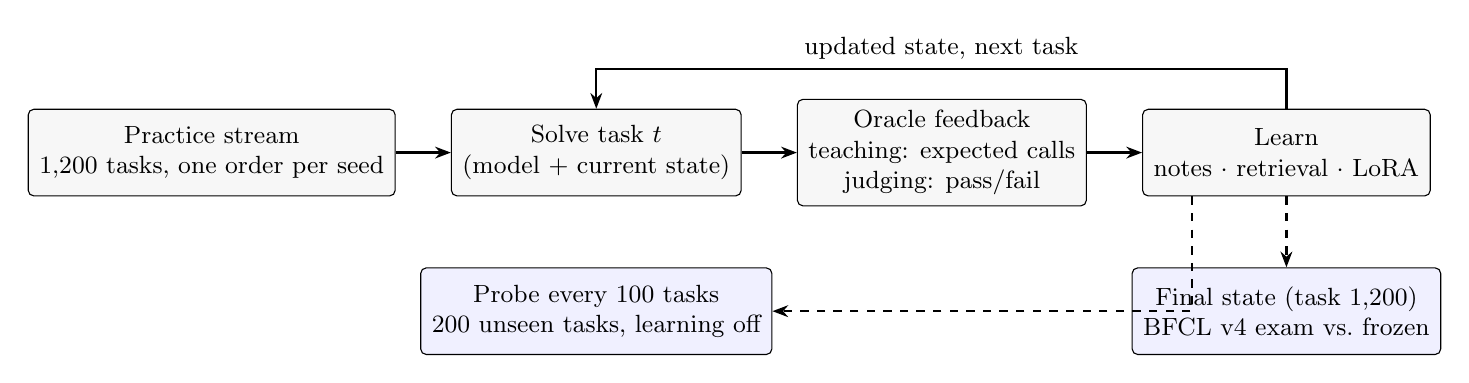
\begin{tikzpicture}[font=\small, node distance=4mm and 7mm,
  box/.style={draw, rounded corners=2pt, align=center, minimum height=11mm, inner sep=4pt, fill=gray!6},
  eval/.style={box, fill=blue!6}, arr/.style={-{Stealth[length=2mm]}, thick}]
\node[box] (stream) {Practice stream\\1,200 tasks, one order per seed};
\node[box, right=of stream] (solve) {Solve task $t$\\(model + current state)};
\node[box, right=of solve] (oracle) {Oracle feedback\\teaching: expected calls\\judging: pass/fail};
\node[box, right=of oracle] (learn) {Learn\\notes $\cdot$ retrieval $\cdot$ LoRA};
\node[eval, below=9mm of solve] (probe) {Probe every 100 tasks\\200 unseen tasks, learning off};
\node[eval, below=9mm of learn] (exam) {Final state (task 1,200)\\BFCL v4 exam vs.\ frozen};
\draw[arr] (stream) -- (solve);
\draw[arr] (solve) -- (oracle);
\draw[arr] (oracle) -- (learn);
\draw[arr] (learn.north) -- ++(0,5mm) -| node[pos=0.25, above]{updated state, next task} (solve.north);
\draw[arr, dashed] (learn.south) ++(-12mm,0) |- (probe.east);
\draw[arr, dashed] (learn) -- (exam);
\end{tikzpicture}
\caption{Study design. Each run practises on the same stream of tasks, in the same order for a given seed; only the learning method and
the feedback differ. The run's state (notes, memory or adapter) is saved every 100 tasks and scored on unseen probe
tasks; its final state takes the official benchmark.}\label{fig:design}
\end{figure*}

\subsection{Practice ground}\label{sec:ground}
We built the practice tasks on BFCL's own multi-turn tools: eight tool classes with executable simulators (a file
system, vehicle control, stock trading, travel booking, support tickets, messaging, social posting and maths), so that
every practice task runs against the same simulators the benchmark uses. An LLM (Gemini 3 Flash) wrote 2,400 multi-turn
tasks in three generations of 800, each refining the last: the first spelled out every step in the user's requests;
the second, like BFCL's questions, left routine steps to the model (changing folder, looking up an identifier, logging
in with credentials given earlier); the third also followed BFCL's mix of tool sets. The writer saw only the tools'
documentation and simulator source code, never BFCL's questions. A task was kept only if its reference calls ran in the
simulators without error, it passed a strict review by the same LLM, and the LLM, solving it through the simulators
without seeing the reference, passed it as BFCL scores it. Fig.~\ref{fig:task} shows one task. Each task gives the simulators' initial state, two to six user turns, and reference calls for each turn (one
to four). Turns per task and calls per turn are drawn, within these ranges, from the distributions counted in the answer file of
BFCL v4's multi-turn base category, and in the third generation the tool sets follow BFCL's composition: four main
sets (file system, vehicle control, trading, travel), each used alone or with one companion set.

\begin{figure}[t]
\centering\small
\fbox{\parbox{0.94\columnwidth}{\raggedright
\textbf{Tools:} vehicle control. \textbf{Initial state:} fuel level 12.5, all four doors locked, brake pedal pressed,
tyre pressures set.\\[4pt]
\textbf{User, turn 1:} ``I'm heading out on a long drive. Tell me how much fuel is in the tank and check if my tire
pressure is healthy.''\\
\textbf{Reference:} {\ttfamily displayCarStatus(option="fuel")}; {\ttfamily check\_tire\_pressure()}\\[4pt]
\textbf{User, turn 2:} ``Everything looks good. Please start the engine so I can get going.''\\
\textbf{Reference:} {\ttfamily startEngine(ignitionMode="START")}}}
\caption{A practice task (second generation). After each turn, BFCL's checker compares the simulator's state with the
state the reference calls produce, and checks that the tools' responses to the reference calls are among those to the
model's calls. The retrieval method shows a logged task to the model in this form: each user request followed by its
calls.}\label{fig:task}
\end{figure}

A task is scored with BFCL's own multi-turn checker against its hidden reference answers, so ``pass'' means here what it
means on the benchmark: after every turn the simulators' state matches the reference's and the responses contain what
the reference requires. The pool is split once and for all (seed 15): the first 1,200 tasks of the shuffled pool form the practice
stream, in that order, and the other 1,200 are held out, of which 200 (67, 67 and 66 from the three generations) form
the probe set used to measure learning on unseen tasks. Probe tasks come from the same generator as the practice tasks,
so the probe measures learning within that distribution; the BFCL exam (Section~\ref{sec:measures}) measures transfer
beyond it.

To check that probe tasks are not near-copies of practice tasks \citep{golchin2024time}, we embedded the user requests of
every task with the sentence encoder used for retrieval (Section~\ref{sec:methods}) and found, for each probe task, the
most similar practice task: the median cosine similarity is 0.68 (maximum 0.90), the same as between a practice task
and its closest other practice task (0.68, maximum 0.92), so the probe tasks are no closer to the practice stream than
its own tasks are to each other. Two of the 200 probe tasks share an
exact reference answer with a practice task, and 4.5\% share the same sequence of functions.

\subsection{Models and harness}\label{sec:models}
We study six instruction-tuned models from five developers, of 0.8B to 1.7B nominal parameters
(Table~\ref{tab:models}). We chose the smallest current instruction-tuned models of open families that BFCL and vLLM can
serve, so that together they range from models that solve no multi-turn question to one that solves a fifth of them, and
we include one reasoning model, Qwen3-1.7B, which writes its reasoning in a \emph{think block} before answering. Each
model runs through a BFCL \emph{handler}, the adapter that writes the tools into the prompt and parses calls from the
reply in the format the model expects: native function calling for four models, and calls written as text for
Gemma-3-1B. BFCL had no handler for LFM2.5 and Qwen3.5, so we wrote handlers that follow their chat templates. Models are
served by vLLM \citep{kwon2023efficient} and decode near-greedily: BFCL sets temperature 0.001, which vLLM raises to its
minimum of 0.01.

BFCL v4 has four groups of questions, each scored by its own checker. \emph{Non-live} questions are single-turn requests
written by BFCL's authors (one, several or parallel calls); \emph{live} questions are single-turn requests contributed by
users. Both include \emph{irrelevance} questions, where no offered tool fits and the right answer is to make no call.
\emph{Multi-turn} questions are conversations against the stateful simulators, in a base form and three harder variants
(a missing function, a missing parameter, a long context); \emph{memory} questions require the model to store and later
recall information through memory tools. Our practice tasks are built for multi-turn base, the \emph{target category}.
We examine every category except web search, which needs a paid search service. Table~\ref{tab:models} gives each
model's frozen scores; for Falcon3-1B, whose leaderboard entry is public, our harness reproduces it (11.1 overall).
Three models, Llama-3.2-1B, Falcon3-1B and Gemma-3-1B, solve no multi-turn question when frozen: they are below the
floor, and they let us test whether a method can lift a model that starts at zero.

\begin{table*}[t]
\centering
\caption{Models and their frozen BFCL v4 scores (\%). Overall: as BFCL weights it, without web search; multi-turn: mean
of its four categories. Parameters: total in the released weights, embeddings included. Handler: BFCL's own (FC: native
function calling; prompt: calls written in text) or ours. Sources:
\citep{yang2025qwen3,amini2025lfm2,liquidai2026introducing,qwenteam2026qwen35,meta2024llama32,falconllmteam2024falcon,gemmateam2025gemma}.}\label{tab:models}
\small
\begin{tabular}{@{}lllrrrrrrr@{}}
\toprule
Model & Developer & Handler & Params & Overall & Non-live & Live & Multi-turn & Multi-turn base & Memory \\
\midrule
Qwen3-1.7B$^{\ast}$ & Alibaba   & BFCL, FC     & 2.03B & 30.0 & 83.9 & 73.9 & 15.9 & 20.0 & 8.4 \\
LFM2.5-1.2B         & Liquid AI & ours         & 1.17B & 23.9 & 67.4 & 63.8 &  4.5 &  9.0 & 7.1 \\
Qwen3.5-0.8B        & Alibaba   & ours         & 0.87B & 20.7 & 47.3 & 56.8 &  5.4 &  8.5 & 4.5 \\
Llama-3.2-1B        & Meta      & BFCL, FC     & 1.24B & 10.7 & 37.9 & 11.8 &  0.0 &  0.0 & 2.6 \\
Falcon3-1B          & TII       & BFCL, FC     & 1.67B & 11.1 & 10.0 &  3.0 &  0.0 &  0.0 & 5.4 \\
Gemma-3-1B          & Google    & BFCL, prompt & 1.00B &  7.1 & 20.0 & 11.8 &  0.0 &  0.0 & 3.2 \\
\bottomrule
\end{tabular}
\par\smallskip{\footnotesize $^{\ast}$Reasoning model (writes a think block before answering).}
\end{table*}

\subsection{The learning loop and feedback}\label{sec:loop}
A run solves the 1,200 practice tasks one at a time in the fixed order. After each task the oracle gives feedback and the
learning method takes it in: notes and retrieval update the run's state at once, LoRA every 10 tasks
(Section~\ref{sec:methods}); the next task uses the updated state. The oracle holds each task's reference calls and runs
BFCL's checker, and its feedback is one of two kinds. Under \emph{oracle teaching} the method receives the expected calls
of every task; the notes method, which learns by reflecting on its attempt, also receives whether the task passed and
the checker's message. Under \emph{oracle judging} the method receives only whether the task passed. In deployment,
teaching stands for a user or supervisor who shows what should have been done, and judging for a signal of success
alone, such as a user's confirmation or a check that the intended effect happened. A \emph{frozen} run learns nothing;
it solves all 2,400 tasks once and is the reference against which every learning run is compared, task by task.

The oracle makes the feedback perfect: the study measures the most each method can learn from a correct signal, its
learning potential, rather than a deployable system that must judge itself (Section~\ref{sec:limits}). Each method takes
the feedback in its own form: the notes method reads it with a transcript of its attempt and writes a lesson, the
retrieval method stores the calls, and LoRA trains on them.

\subsection{Learning methods}\label{sec:methods}
All three methods are meant to run on the device itself: none needs a larger model or an external service, and none
changes the base weights. Notes and retrieval need only the model's own inference, plus one extra generation per task
for notes to write the lesson; LoRA also needs training, whose cost we report in Section~\ref{sec:res-cost}. In
knowledge-systems terms, the three keep what is learned in three forms: as explicit rules the model writes for itself
(notes), as stored cases retrieved by similarity, as in case-based reasoning \citep{aamodt1994case} (retrieval), and as
parameters (LoRA). Their settings are listed in Table~\ref{tab:settings}; the exact prompts are in the released
code (Section~\ref{sec:compute}). The settings were fixed before the full runs, from common practice and from the
practical limits found in pilots (memory, time per task); none was tuned on the probe set or on the benchmark.

\begin{table*}[t]
\centering
\caption{Settings of the three learning methods and of the reasoning-kept arm.}\label{tab:settings}
\small
\begin{tabular}{lll}
\toprule
Method & Setting & Value \\
\midrule
\multirow{4}{*}{Notes}
 & Lesson & one per task, written by the model from its attempt and the feedback (under 30 words) \\
 & Repeats & a lesson overlapping a kept note by word Jaccard $\ge 0.6$ is dropped \\
 & Size limit & 600 tokens; above it the model merges and trims its notes \\
 & Placement & one system message at the start of every task \\
\midrule
\multirow{5}{*}{Retrieval}
 & Memory & every task (teaching) or every passed task (judging), logged verbatim \\
 & Encoder & all-MiniLM-L6-v2 \citep{wang2020minilm,reimers2019sentence}, 22M parameters, on the CPU \\
 & Candidates & logged tasks using the same tool classes, ranked by cosine similarity of the user requests \\
 & Examples & up to 3 within 1,200 tokens (600 in a budget check for Qwen3-1.7B) \\
 & Placement & one system message at the start of every task \\
\midrule
\multirow{6}{*}{LoRA}
 & Adapter & rank 16, $\alpha$ 32, no dropout, on the attention and MLP projections (see text) \\
 & Optimiser & AdamW, learning rate $10^{-4}$, batch 1, 4-step gradient accumulation, clipping 1.0 \\
 & Update & every 10 tasks: one pass over new examples plus replayed ones \citep{rolnick2019experience}, $2\times$ as many \\
 & Loss & answer tokens only; examples over 12,288 tokens skipped \\
 & Serving & new adapter hot-loaded into vLLM after each update (120 updates in a teaching run) \\
 & Targets & teaching: expected calls in the model's format; judging: the model's own passed attempts \\
\midrule
\multirow{4}{*}{\shortstack[l]{LoRA,\\reasoning\\kept}}
 & Training & as LoRA teaching (Qwen3-1.7B only) \\
 & Reasoning & written by the base model at each step, given the expected reply as a hint \\
 & Length & at most 512 tokens, cut at the last full sentence \\
 & Filter & sentences that mention the hint dropped; trained on with the calls \\
\bottomrule
\end{tabular}
\end{table*}

\subsubsection{Self-written notes}
The notes start empty. After each task, the same model reads a transcript of its attempt (the user turns, its calls and
the tools' replies) and the feedback, and writes one lesson of under 30 words, sampled at temperature 0.7. A lesson that
mostly repeats a note already kept is dropped. The notes go into a system message at the start of every task; above
the size limit, the model rewrites them as at most 12 bullet points, and if they are still too long, the oldest notes
are dropped. This follows the design of an evolving
cheatsheet that the model curates itself \citep{suzgun2026dynamic}.

\subsubsection{Retrieved experience}
The memory starts empty. Every finished task is logged verbatim, with its tool classes, the user's request in each turn,
and the calls: the expected calls of every task under teaching, and the model's own calls of passed tasks only under
judging. Before each task, the logged tasks that use the same tool classes are ranked by the cosine similarity of their
user requests to the new task's, embedded with a small sentence encoder \citep{wang2020minilm,reimers2019sentence};
the top tasks within the budget go into a system message as worked examples, with calls written in BFCL's reference
syntax. Whole tasks are used, not summaries, as in trajectory-as-exemplar prompting \citep{zheng2024synapse}.

\subsubsection{Continual LoRA}
A LoRA adapter \citep{hu2022lora} is trained every 10 tasks on the examples gathered since the last update, together
with replayed earlier examples \citep{rolnick2019experience}, and then loaded into the running vLLM server, so that the
next task uses it. The adapter targets the attention and MLP projections by their standard names; in LFM2.5 only the
query, key and value projections carry these names, and Qwen3.5's linear-attention layers have none, so those parts
are not adapted.

Under teaching, the training examples are the expected calls written in the model's own tool-call format. To obtain
exactly the prompts the model would see, including the tools' outputs, the expected calls of each turn are replayed
through the model's own handler with a stand-in for the model that returns them as its answers; the resulting prompt--answer pairs are
the examples. Each turn ends with a scripted closing reply, also trained on, so that the model learns to end a turn: in
a pilot without it, the model kept calling tools until the turn was cut off. Before any run we checked 30 tasks per
model: every replay passed the checker, and for the four models with BFCL's own handlers every rendered answer decoded
back to the expected calls (our two handlers parse calls only while querying, so this check does not apply to them). For Qwen3-1.7B the
targets open with an empty think block, which is kept out of the loss.

Under judging, the examples are the model's own prompts and answers from tasks that passed, its reasoning included: a
form of self-imitation \citep{oh2018self,zelikman2022star}. A model that passes no task learns nothing.

\subsubsection{Teaching with the reasoning kept}
Training a reasoning model on targets with an empty think block may teach it to stop reasoning, besides teaching it the
calls. To separate the two, a third LoRA arm for Qwen3-1.7B keeps reasoning in the targets. At each step of the replay,
the base model (not the adapter) sees the conversation so far and a one-off hint showing the correct next reply, and is
asked to reason briefly about why that reply is right without mentioning the hint, as in STaR's rationalization
\citep{zelikman2022star}. The reasoning is capped at 512 tokens, cut at the last full sentence, and stripped of any
sentence that mentions the hint; it opens the target and is trained on with the calls. Because it is written during the
replay, later steps of a turn see the reasoning of earlier steps, as they would when the model answers for itself.

\subsection{Runs}\label{sec:runs}
Table~\ref{tab:runs} lists the runs. Seed 15 practises in the split's order; seeds 16 and 17 practise on the same 1,200
tasks in other orders, with the probe set and exam unchanged. The seed also sets the random choices made while learning:
which earlier examples LoRA replays, and the sampling of lessons in the notes method. Three seeds were run where the main claims rest: LoRA teaching
for every model except Falcon3-1B, whose single run supports the same claim as Llama's and Gemma's; both LoRA arms of
Qwen3-1.7B; and the reasoning-kept arm. Every other cell has one seed (15). LoRA and retrieval runs that learn nothing
(judging for models that pass no practice task) end as the frozen model and are not examined again.

\begin{table}[t]
\centering
\caption{Runs. Every learning run practises on the same 1,200 tasks; the frozen runs solve all 2,400. T: oracle
teaching; J: oracle judging. Three seeds for the six LoRA cells the main claims rest on and for the reasoning-kept
arm; retrieval adds a 600-token-budget run for Qwen3-1.7B.}\label{tab:runs}
\small
\begin{tabular}{@{}llrl@{}}
\toprule
Method & Arms & Runs & Seeds \\
\midrule
Frozen                 & --           & 6  & 15 \\
Notes                  & T, J         & 12 & 15 \\
Retrieval              & T, J         & 13 & 15 \\
LoRA                   & T, J         & 24 & 15--17 \\
LoRA, reasoning kept   & T (Qwen3)    & 3  & 15--17 \\
\bottomrule
\end{tabular}
\end{table}

\subsection{Measures}\label{sec:measures}
We measure learning in three ways. \emph{Gain over frozen} compares each practice task's result with the frozen run's on
the same task, so that differences in task difficulty cancel; we report it over all 1,200 tasks. Because it averages
over the whole stream, including the early tasks before anything was learned, it understates what the final state can do;
the probe measures that.
The \emph{probe curve} scores the run's state saved every 100 tasks (its notes, memory or adapter) on the 200 probe tasks
with learning turned off, giving 13 points per run including the base model. The \emph{BFCL exam} scores the final state
(task 1,200) on the BFCL v4 exam with the same harness as the frozen models: notes go into the prompt of every question,
as they were in every practice task;
retrieved examples go into multi-turn questions, the only ones with logged tasks that use the same tools; adapters are
merged into the weights. We report the change against the frozen score in every category, with multi-turn base as the
target. Outside multi-turn we separate questions that need a call from
questions where no tool fits and the right answer is to make none (BFCL's irrelevance questions), because the two can
move in opposite directions. Together, these gains under oracle feedback are our measure of a method's learning
potential for a model.

\subsection{Statistical analysis}\label{sec:stats}
Every comparison is paired: the same tasks or questions, solved or not, under two conditions. A single run is compared
with its reference (the frozen model on practice, the start on the probe, the frozen score on BFCL), and LoRA with retrieval and
retrieval with notes for the same model and arm, with McNemar's exact test on the discordant pairs
\citep{mcnemar1947note,dietterich1998approximate} and a 95\% paired bootstrap interval over tasks or questions
\citep{efron1993introduction}. For cells with three seeds we report the mean over seeds, test it with a paired sign-flip
test of the per-question seed mean, and give a bootstrap interval over questions. Tests are corrected with Holm's method
\citep{holm1979simple} within each family: all runs against their frozen score on BFCL multi-turn base, the same in BFCL's other
groups, all runs on the probe, all runs on practice, the method comparisons, and the three-seed cells.

\subsection{Implementation and compute}\label{sec:compute}
We used bfcl-eval 2026.3.23, vLLM 0.8.5 for four models (the version bfcl-eval pins) and vLLM 0.33 or
0.34 for LFM2.5 and Qwen3.5 (the latest release when each machine was set up), and PEFT \citep{mangrulkar2022peft} for LoRA. Each run used one NVIDIA L4 (24\,GB) or A100
(40\,GB) GPU on Google Cloud, which runs of the same model sometimes shared; under LoRA, the vLLM server used about half of the GPU's memory and the trainer
the rest. A run took between 1.4 and 34 hours. The code, including every prompt, the practice tasks, the split and the per-question results of every run
are openly available, with the full run logs and adapters archived separately (see Data availability).

%% ---------------------------------------------------------------------------------------------------------------
\section{Results}\label{sec:results}
We report each method in turn (Sections~\ref{sec:res-notes}--\ref{sec:res-reasoning}), in the order of
Section~\ref{sec:methods}, then compare them (Section~\ref{sec:bfcl}) and give their cost (Section~\ref{sec:res-cost}).
For each method we give the gain over the frozen model on practice, the change on the probe, the change on BFCL
multi-turn base against the frozen score, and any significant change in BFCL's other groups. Three-seed cells are reported as
the mean with a 95\% interval over questions, single runs as the change with McNemar's $p$; ``significant'' means a
Holm-adjusted $p<0.05$ within its family of tests (Section~\ref{sec:stats}).

Frozen, the six models span the range the study needs. On the practice tasks Qwen3-1.7B solves 52.8\%, LFM2.5 30.0\%
and Qwen3.5 25.9\%; on the probe they start at 51.0\%, 26.0\% and 25.5\%. Llama, Falcon and Gemma solve none, and
they fail in a different way. A multi-turn task fails at its first wrong turn, and for Llama and Gemma that is a turn in
which they make no call at all, in 99.3\% and 99.8\% of the 2,400 practice tasks. Instead of calling a tool they answer
in prose or write code: asked on BFCL to find files, Llama named the function to use and then wrote its own Python
function instead of calling it. Falcon either makes no call (37\%) or fails with errors from overrunning its short
context window (60\%). The models above the floor fail mostly by calling wrongly: LFM2.5 and Qwen3-1.7B leave the wrong
state or responses in 62\% and 39\% of the tasks, and Qwen3.5 keeps calling until the turn is cut off in 31\%.


\subsection{Self-written notes}\label{sec:res-notes}
\begin{figure*}[t]
\centering
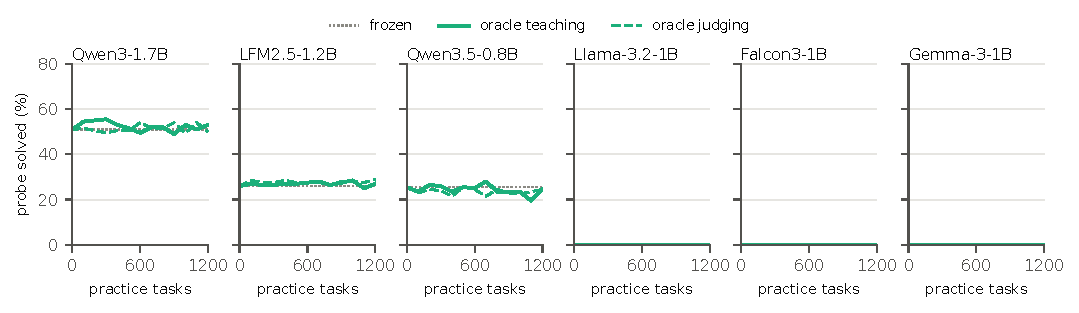
\includegraphics[width=\textwidth]{figures/notes_curves.pdf}
\caption{Self-written notes: probe score every 100 practice tasks. Solid: oracle teaching; dashed: oracle judging;
dotted: the frozen model. Figs.~\ref{fig:retrieval} and~\ref{fig:lora} use the same layout and scale.}\label{fig:notes}
\end{figure*}
Notes produced no measurable learning (Fig.~\ref{fig:notes}). Against the frozen model on the same practice tasks, no
run changed by more than 3.4 points and none significantly; on the probe every run ended within 3 points of its start,
and on BFCL multi-turn base within 2 points of its frozen score.

The lessons show why. In every run, 70 to 100\% of them named no tool or function at all; they were maxims such as
``Always validate tool parameters before execution to ensure accuracy'' (LFM2.5) or ``Carefully analyze instructions
before executing any tool'' (Gemma). By the method's own overlap test, 27 to 96\% of lessons nearly repeated one of the
previous 50, so the notes, held under 600 tokens, cycled through a few such rules. Where a lesson was specific, it could
be wrong: 18 of the 27 lines in Qwen3.5's final notes under teaching told it, in different words, to ``verify
credentials via \texttt{pwd()} before every API call'', although \texttt{pwd} only prints the current folder. The three
models below the floor passed no practice task with or without notes, so their lessons never drew on a success.

Notes did shift the balance between calling and abstaining, because they enter every BFCL prompt, single-turn questions
included: LFM2.5 and Qwen3.5 called more and abstained less (Qwen3.5 under teaching abstained correctly 71 points less
often), while Llama and Gemma called less and abstained more.

\subsection{Retrieved experience}\label{sec:res-retrieval}
\begin{figure*}[t]
\centering
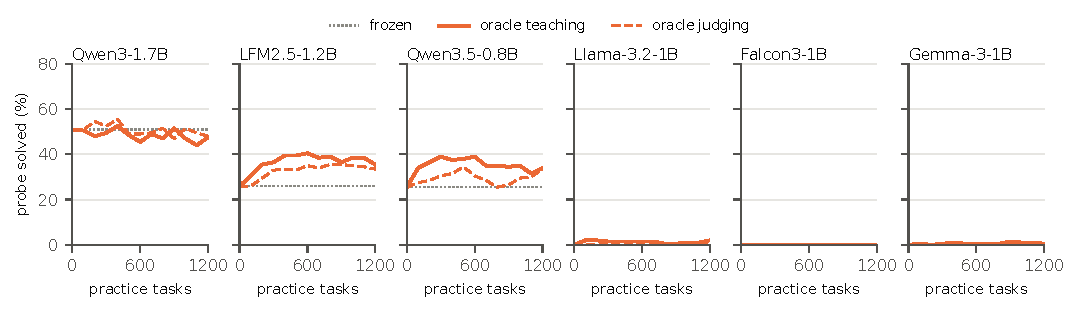
\includegraphics[width=\textwidth]{figures/retrieval_curves.pdf}
\caption{Retrieved experience: probe score every 100 practice tasks, in the layout of Fig.~\ref{fig:notes}.}
\label{fig:retrieval}
\end{figure*}
Retrieval helped while practising: the gain over frozen was significant for LFM2.5 under teaching (+9.1 points) and for
Qwen3.5 under teaching and judging (+13.9, +8.6), small but significant for Llama and Gemma (+1.0, +1.2), and
negative for Qwen3-1.7B under teaching ($-$6.0). On the probe the changes were of similar size for LFM2.5 (+9.5) and
smaller for Qwen3.5 (+8.5), but with 200 tasks instead of 1,200 neither was significant after correction
(Fig.~\ref{fig:retrieval}). On BFCL multi-turn base, LFM2.5 and Qwen3.5 gained 3.5 to 5.5 points, none significant
(best: LFM2.5 teaching, +5.5, $p=0.019$ before correction).

The examples are written in BFCL's reference syntax rather than in each model's own call format, so a model must
carry them over into its own. For Qwen3-1.7B, whose prompts were already the longest because of its reasoning, they
lowered practice by 6 points. Halving the budget to 600 tokens, to test whether prompt length was the limit, reduced
that loss to 2.7 points and changed nothing significantly on the probe or on multi-turn base. Outside multi-turn,
retrieval changed nothing it could change: single-turn and memory questions use other tools and receive no examples,
so the model there is the frozen one, and its scores moved only by run-to-run variation (Section~\ref{sec:limits}).

\subsection{Continual LoRA}\label{sec:res-lora}
\begin{figure*}[t]
\centering
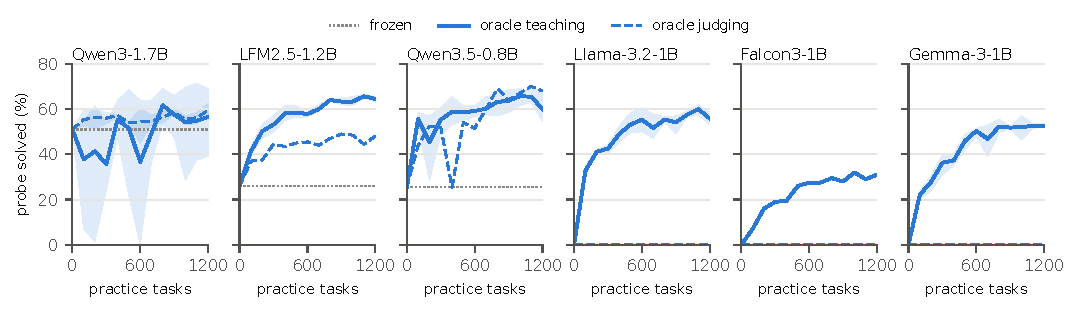
\includegraphics[width=\textwidth]{figures/lora_curves.pdf}
\caption{Continual LoRA: probe score every 100 practice tasks, in the layout of Fig.~\ref{fig:notes}. Cells with three
seeds show the seed mean with the range shaded (teaching: all but Falcon; judging: Qwen3-1.7B). Under judging the
models below the floor pass no task and learn nothing.}\label{fig:lora}
\end{figure*}
Under teaching, LoRA produced the largest gains on our tasks (Fig.~\ref{fig:lora}). Over three seeds, the gain over frozen across the 1,200 practice tasks was
+49.4 points for Llama, +41.6 for Gemma, +36.2 for Qwen3.5 and +29.1 for LFM2.5, and the probe rose by +55.8, +52.7,
+34.5 and +38.5; Falcon, with one seed, rose by +31 on the probe. All of these are significant. On BFCL multi-turn base
the picture changes: Llama (+10.3, interval 6.8 to 14.0) and Gemma (+11.0, 7.3 to 15.0) gained significantly in every
seed, but LFM2.5 (+3.5), Qwen3.5 (+5.7, $p=0.024$ before correction) and Falcon (+3, one seed) did not. Qwen3.5's three
seeds also differed on the probe (54.5 to 68.5 at task 1,200; one seed fell to 28.5 at task 200 and recovered).

Under judging, LoRA learned where the model already passed tasks: the probe rose significantly for LFM2.5 (+22) and
Qwen3.5 (+42.5), while their BFCL gains (+4.5 and +9) were not significant after correction. The models below the floor,
passing no task, learned nothing.

\begin{figure*}[t]
\centering
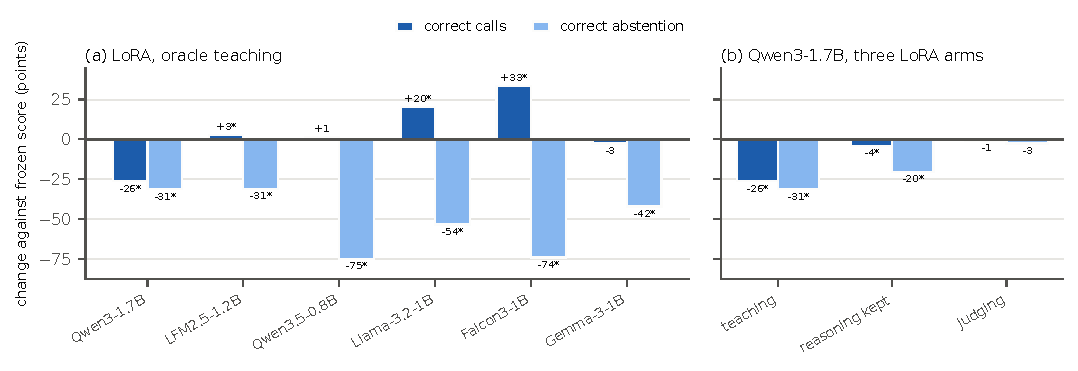
\includegraphics[width=\textwidth]{figures/overcalling.pdf}
\caption{Over-calling after LoRA: change against the frozen score in BFCL's single-turn and live questions that need a call
(correct calls) and in those where no tool fits and the right answer is no call (correct abstention). (a) Oracle teaching,
all six models; (b) Qwen3-1.7B under the three LoRA arms. Seed 15 for every bar. *: significant (McNemar's test,
Holm-corrected). Every run, measure and test is in the released data.}
\label{fig:overcalling}
\end{figure*}
LoRA changed behaviour outside multi-turn in one consistent way (Fig.~\ref{fig:overcalling}a): every model learned to
call a tool even when none fitted. Correct abstention fell by 31 to 75 points for all six models under teaching, and by
30 for LFM2.5 and 63 for Qwen3.5 under judging, all significant. Asked ``How many calories does an apple have?'' with
only a tool for estimating litigation costs on offer, frozen Llama replied that it had no function for this; after LoRA
teaching it called {\ttfamily calculate\_litigation\_cost(length\_in\_days=5, complexity='low')}. At the same time
correct calls rose for Llama (+20) and Falcon (+33). Separately, memory scores fell significantly under teaching for four
models, by 4.5 to 8 points, to zero for Qwen3.5 in every seed.

\subsection{Teaching with the reasoning kept}\label{sec:res-reasoning}
For Qwen3-1.7B we compare keeping the reasoning with the two other LoRA arms, plain teaching and judging
(Table~\ref{tab:arms}, Fig.~\ref{fig:reasoning}). The three arms diverged.

Plain teaching on expert calls made learning erratic. The probe ended between $-$12 and +18 points from its start,
depending on the seed, practice fell by 5.8 points against the frozen model, and BFCL's live and non-live scores fell in
every seed: the model lost correct calls ($-$26) as well as correct abstention ($-$31) in seed 15
(Fig.~\ref{fig:overcalling}b). Keeping the reasoning in the targets made learning steady, with the three seeds within
about 3 points of each other, and cut the losses in live and non-live by more than half. But this arm was the only one to
lower multi-turn base significantly, by 8.2 points (7 to 9 in every seed). Judging, on the model's own passed attempts
with its own reasoning, raised the probe by 8.5 points and lowered no BFCL group significantly in any seed.

\begin{table}[t]
\centering
\caption{Qwen3-1.7B under the three LoRA arms: change in points, mean over three seeds (calls and abstention: seed 15).
Practice against the frozen model, probe against the start, BFCL against the frozen score. *: significant (three-seed
cells: sign-flip test; BFCL groups: in every seed; calls and abstention: McNemar's test). Seed standard deviation of the
probe change: 15.6, 1.3 and 2.6. Memory changes of a few points are within run-to-run variation
(Section~\ref{sec:limits}).}\label{tab:arms}
\small
\begin{tabular}{@{}lrrr@{}}
\toprule
Measure & Teaching & Reasoning kept & Judging \\
\midrule
Practice                & $-$5.8*  & +7.4*    & +2.8   \\
Probe                   & +5.5     & +11.0*   & +8.5*  \\
Multi-turn base         & $-$4.3   & $-$8.2*  & +3.0   \\
Live                    & $-$26.1* & $-$12.0* & $-$1.3 \\
Non-live                & $-$20.3* & $-$5.5*  & $-$0.5 \\
Memory                  & $-$7.3*  & +1.4     & +5.0   \\
Correct calls           & $-$26*   & $-$4*    & $-$1   \\
Correct abstention      & $-$31*   & $-$20*   & $-$3   \\
\bottomrule
\end{tabular}
\end{table}

\begin{figure}[t]
\centering
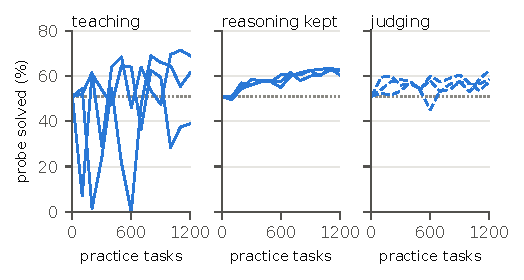
\includegraphics[width=\columnwidth]{figures/reasoning_curves.pdf}
\caption{Qwen3-1.7B under the three LoRA arms: probe score every 100 practice tasks, one line per seed, on the scale
of Figs.~\ref{fig:notes}--\ref{fig:lora}; dotted: the frozen model.}
\label{fig:reasoning}
\end{figure}

\subsection{The methods compared}\label{sec:bfcl}
Table~\ref{tab:bfcl} puts the methods side by side on BFCL multi-turn base. On the probe, LoRA beat retrieval
significantly for LFM2.5 and Qwen3.5 under both arms and for the three models below the floor, by 14.5 to 56.5 points; for
Qwen3-1.7B the two did not differ significantly, and retrieval and notes could not be told apart after correction. On BFCL multi-turn base, LoRA
beat retrieval only for Llama (+8) and Gemma (+11); for LFM2.5 and Qwen3.5 the two were indistinguishable ($-$3.5 to
+4, all $p>0.16$), and for Qwen3-1.7B under teaching LoRA was significantly worse ($-$10). Outside multi-turn, LoRA moved
every model from abstaining towards calling (Fig.~\ref{fig:overcalling}), retrieval left the balance unchanged, and notes
moved it in either direction (Section~\ref{sec:res-notes}).

\begin{table*}[t]
\centering
\caption{BFCL v4 multi-turn base: change against the frozen score (points). T: oracle teaching; J: oracle judging. Three-seed
cells: mean [95\% interval over questions]; other cells: seed 15. *: significant after Holm correction. --: not examined
(nothing learned, so the final state is the frozen model). Retrieval with a 600-token budget for Qwen3-1.7B: $-$3.0.}
\label{tab:bfcl}
\small
\begin{tabular}{lrrrrrrrr}
\toprule
& & \multicolumn{2}{c}{Notes} & \multicolumn{2}{c}{Retrieval} & \multicolumn{2}{c}{LoRA} & \\
\cmidrule(lr){3-4}\cmidrule(lr){5-6}\cmidrule(lr){7-8}
Model & Frozen (\%) & T & J & T & J & T & J & Reasoning kept \\
\midrule
Qwen3-1.7B   & 20.0 & $-$2.0 & +1.0 & +1.0 & +3.0 & $-$4.3 [$-$9.7, 0.8] & +3.0 [$-$1.7, 7.7] & $-$8.2* [$-$13.0, $-$3.5] \\
LFM2.5-1.2B  &  9.0 & +1.0 & +1.5 & +5.5 & +3.5 & +3.5 [$-$0.8, 8.2] & +4.5 & \\
Qwen3.5-0.8B &  8.5 & +1.0 &  0.0 & +4.0 & +5.0 & +5.7 [1.0, 10.5] & +9.0 & \\
Llama-3.2-1B &  0.0 &  0.0 &  0.0 &  0.0 & -- & +10.3* [6.8, 14.0] & -- & \\
Falcon3-1B   &  0.0 &  0.0 &  0.0 &  0.0 & -- & +3.0 & -- & \\
Gemma-3-1B   &  0.0 &  0.0 &  0.0 & +0.5 & -- & +11.0* [7.3, 15.0] & -- & \\
\bottomrule
\end{tabular}
\end{table*}



\subsection{Cost}\label{sec:res-cost}
Measured on server GPUs, the methods differ in where their cost falls. Notes and retrieval need no training but lengthen
every prompt: notes by 160 to 540 tokens (0.9--3.3\,KB, capped) and retrieval by up to 1,200 tokens; retrieval's memory
also grows with every task, to 1.26\,MB after 1,200, and notes need one extra generation per task to write the lesson. A
practice task took 4 to 10\,s with either method on a shared L4, except for the reasoning model (79\,s with notes on an
L4, 24\,s with retrieval on an A100). LoRA adds nothing to the prompt once its 3.5--70\,MB adapter is merged, but training
dominates its time: under plain teaching, training took 70 to 98\% of each practice task's time, and one update, every
10 tasks, took 1 to 16 minutes on a dedicated A100 (LFM2.5 fastest, Qwen3.5 slowest). On a phone or laptop these updates
would take longer and would have to run while the device is idle. The cost of every run is in the released data
(Section~\ref{sec:compute}).

\section{Discussion}\label{sec:discussion}
We take the four research questions in turn: whether a method can lift a model from zero (RQ1,
Section~\ref{sec:floor}), what else changes when a model learns, in general and in a reasoning model (RQ2,
Sections~\ref{sec:side} and~\ref{sec:reasoningft}), how far the gains reach beyond the practice tasks (RQ3,
Section~\ref{sec:transfer}), and which feedback suits which model (RQ4, Section~\ref{sec:teachjudge}). We then set out
the limits of the study (Section~\ref{sec:limits}) and, given them, the implications for practice
(Section~\ref{sec:guidance}).

\subsection{Only LoRA lifts models from zero}\label{sec:floor}
RQ1 has the clearest answer, and it reveals a floor: only weight updates lifted a model that could not yet do the task.
Models that make no valid multi-turn call gained nothing from their own notes and at
most a point on practice from correct worked examples of the same tools, with nothing on unseen tasks, yet continual
LoRA lifted all three on our tasks and two of them, Llama and Gemma, on the official benchmark. We read this as a
minimum competence that in-context learning needs and that weights can supply: Llama and Gemma failed almost every task
by producing no call at all, answering in prose or writing code instead, so an example of the right call had nothing to
build on, whereas LFM2.5, which already produced calls, did gain from retrieval while practising.

Two other explanations fit less well. Retrieved examples are written in BFCL's reference syntax rather than in each
model's own call format, so a weak model might simply fail to carry them over; but the notes, which are plain advice,
failed as completely, and LoRA, which trains on the model's own format, succeeded. Falcon's prompts overran its short
context, which may explain why its BFCL gain was smaller than Llama's and Gemma's; but Llama and Gemma failed by not
calling, not by running out of room. In-context learning is known to grow with model size \citep{brown2020language},
and the floor may be where that ability runs out for a given task.

The floor also reverses what earlier comparisons found for other kinds of learning, where the context route did as well as
fine-tuning or better: few-shot fine-tuning and in-context learning generalised similarly \citep{mosbach2023few}, and
retrieval beat fine-tuning for injecting knowledge \citep{ovadia2024fine,soudani2024fine}. For a procedural skill in a
small model, weights were the only route that worked below the floor. Self-written notes, which improved large models in
the cheatsheet and playbook designs \citep{suzgun2026dynamic,zhang2026agentic}, did not help any model at this scale; the
generic, repeated lessons of Section~\ref{sec:res-notes} are an extreme form of the brevity bias and context collapse
that Zhang et al.~\citep{zhang2026agentic} describe in evolving contexts. LifelongAgentBench found that replaying past
experience in the prompt helps agents little, because of irrelevant information and limited context
\citep{zheng2025lifelongagentbench}; in small models we see the same limit more sharply, as retrieved examples gave
significant gains only on practice and lowered practice for Qwen3-1.7B, whose prompts were already the longest. Which route is open to a small model is
therefore decided before any choice of method, and a frozen check on a few tasks tells which.

\subsection{Side effects of learning}\label{sec:side}
On RQ2, learning changed more than the skill being practised. The largest change was not a lost skill but a changed habit
(Fig.~\ref{fig:overcalling}): after LoRA teaching, every model called a tool when none fitted, losing 31 to 75 points
of correct abstention, and LFM2.5 and Qwen3.5 did so under judging too, while Llama and Falcon called correctly more
often. A likely cause is that every practice task asks for calls in every turn, so the training targets never show the
model declining; practice for tool use should include requests that no tool can serve. Function-calling work has met
this problem in offline training: Hammer adds a dataset of irrelevant functions so that small on-device models stay
able to decline \citep{lin2025robust}, and our results show what on-the-job learning does without such data. Nor is this
the forgetting that continual fine-tuning is usually checked for \citep{kirkpatrick2017overcoming,luo2025empirical}.
LoRA with replay \citep{rolnick2019experience}, which forgets less than full fine-tuning \citep{biderman2024lora},
still changed the model's habits, and a check of retained skills alone would have missed it, since correct calls even
rose for two models. Notes shifted the same balance in
either direction, and LoRA also erased Qwen3.5's memory score in every seed. An overall score blurs all of this: a model
that gains on the target category and loses its ability to decline may score the same overall as before. Evaluations of
learning on the job should therefore report each category, with the target named in advance.

\subsection{Fine-tuning reasoning models}\label{sec:reasoningft}
For the reasoning model, the second part of RQ2, what Qwen3-1.7B was trained on mattered more than whether its
reasoning was kept. We expected the empty think
block in the expert targets to be the cause of the harm, by teaching the model to stop reasoning. Keeping the reasoning
steadied learning and cut the damage to other skills by more than half, but did not remove it, and it was the only arm
to lower the benchmark's target category significantly. This suggests that the reasoning it learned to write fitted our
tasks rather than BFCL's. Only training on its own verified successes, in its own words, avoided harm everywhere,
although its benchmark gain was not significant.

A likely reason is distance from the model's own behaviour. Its passed attempts are text it already produces, so
training on them sharpens habits it has; expert calls, and reasoning written for them by a model that was given the
answer, pull it towards outputs it would not produce, and the pull spreads to other skills. This is the logic of
self-imitation and self-training \citep{oh2018self,zelikman2022star}, and our results suggest it matters more for
preserving a model's other skills than for raising its target score. Reasoning is now trained into models directly
\citep{guo2025deepseek,yang2025qwen3}; our results suggest that later fine-tuning on answers alone can undo part of that
training, and that rationalization \citep{zelikman2022star} protects it only in part. These results come from one
reasoning model, and teaching was also variable for Qwen3.5, so the instability is not unique to reasoning models.

\subsection{Small gains on BFCL}\label{sec:transfer}
\begin{figure}[t]
\centering
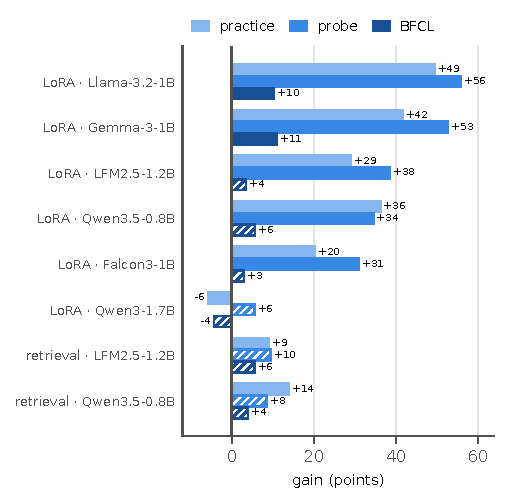
\includegraphics[width=\columnwidth]{figures/transfer.pdf}
\caption{Gain under oracle teaching at three distances from practice: on the practice tasks (against the frozen model),
on the unseen probe tasks (against the start) and on BFCL multi-turn base (against the frozen score). LoRA cells with three
seeds show the seed mean. Solid: significant after Holm correction; hatched: not significant. Not drawn: notes (no
gain at any stage), retrieval for the models below the floor (within about a point of zero), and retrieval for Qwen3-1.7B (practice $-$6.0,
significant; no significant change on the probe or BFCL).}\label{fig:transfer}
\end{figure}
On RQ3, gains reached unseen tasks of the same kind but arrived at the official benchmark smaller than it can resolve,
except for Llama and Gemma. Fig.~\ref{fig:transfer} brings together the gains reported in Section~\ref{sec:results} at three distances from
practice. Retrieval's gains were of similar size on practice and on the probe for LFM2.5, but on 200 probe tasks they
were not significant, and on BFCL they shrank further. LoRA reached unseen tasks, often by more than it gained on
practice, which averages over early tasks before anything was learned, and it was significant there for every arm that
learned except Qwen3-1.7B under plain teaching. On BFCL multi-turn base, however, it was significant only for Llama and
Gemma, two of the three models that started at zero.

The main reason is likely that our tasks are easier than BFCL's, and the frozen models show it: the three that solve any
multi-turn task each solved two and a half to three times as much of our probe as of BFCL multi-turn base (Qwen3-1.7B 51
against 20, LFM2.5 26 against 9, Qwen3.5 25.5 against 8.5). The first of our three generations spelled out every step,
which BFCL leaves to the model, and BFCL's tasks probably also demand longer plans and closer tracking of state. Our tasks
share one generator's style as well, so part of what was learned may be that style rather than the tools. This gap is
the price of never practising on BFCL's own questions, which we avoided because public benchmarks may leak into
training \citep{golchin2024time}. Learning on the
job, for these models, is real but local; practice tasks that are harder, more varied, or calibrated against the
benchmark's difficulty would test how far it can reach. The result is also a lesson about evaluation: for the models above the floor, LoRA's probe
gains of 22 to 42 points arrived at the benchmark at a size its 200 target questions cannot resolve, so a single benchmark
category is too blunt an instrument to judge learning on the job, and a larger held-out test, or one pooled over seeds,
is needed to tell a small gain from none. Benchmarks that score learning along the stream itself
\citep{wu2024streambench,wei2025evomemory} measure the first of our three distances; our results show how much the
other two can change the picture.

\subsection{Teaching vs judging}\label{sec:teachjudge}
On RQ4, the two kinds of feedback suit different starting points. Below the floor only teaching works: judging learns from
passed tasks, and a model that passes none learns nothing. Above it, judging gained no less on the benchmark: under LoRA,
LFM2.5 and Qwen3.5 gained +4.5 and +9 on BFCL multi-turn base by judging against +3.5 and +5.7 by teaching, though no
difference was significant and 200 questions cannot show one below about 5 points either way, even though teaching gained more on our own tasks for LFM2.5 (probe +38.5 against +22). For the
reasoning model, judging was the only arm without harm (Section~\ref{sec:reasoningft}). Judging is not a cure for
over-calling, however: LFM2.5 and Qwen3.5 lost 30 and 63 points of correct abstention under judging too, and Qwen3.5
lost more on BFCL's non-live questions by judging than by teaching ($-$15.5 against $-$4.5). A natural schedule
follows: teach a model until it can succeed, then let it learn from its own verified successes.

\subsection{Limitations and threats to validity}\label{sec:limits}
\emph{Scope.} The oracle makes these results a ceiling, not the behaviour of a deployable system that must judge
itself. The study covers one domain (BFCL's tools, multi-turn), practice tasks written by one LLM, six models of 0.8B to
1.7B nominal parameters, and one reasoning model.

\emph{Statistical power.} With 200 questions, the 95\% intervals on BFCL multi-turn base span about $\pm$5 points and
those on the probe about $\pm$7, so smaller gains cannot be told from zero: ``not significant'' means not shown, not
absent. Most cells have one seed, and the seeds we did run show that a single run can mislead (Qwen3-1.7B under
teaching ended the probe anywhere from $-$12 to +18).

\emph{Measurement noise.} BFCL's answers vary slightly between runs of the same model. Because retrieval adds nothing
to single-turn and memory questions, its exams repeat the frozen model there: a few per cent of answers changed in each
direction (up to 9\% in memory), and the net change stayed within 1.5 points, except in memory for Qwen3-1.7B (+2.6 to
+5.8 over three exams, one of them significant), whose frozen score comes from an earlier run. Changes of a few points
in memory should therefore not be read as effects; the over-calling effects, of 30 to 75 points, are far above this
noise.

\emph{Implementation.} Settings were fixed before the runs and not tuned for any method, and another notes prompt or
retrieval budget might do better. Two of the six handlers are ours, and two models ran on a newer vLLM. LoRA adapts
fewer layers in LFM2.5 and Qwen3.5 than in the other models (Section~\ref{sec:methods}), and retrieved examples use
BFCL's reference syntax rather than each model's own format. Costs were measured on server GPUs (L4 and A100), shared
in different ways, so they compare the methods but do not give on-device times. Adapters were hot-loaded during
practice and merged into the weights for the exam; the two are mathematically equivalent, but we did not check that they
give identical outputs.

\subsection{Implications for practice}\label{sec:guidance}
Given these limits, the results suggest four implications for systems that learn tool use on the job. They come from six models, one domain and oracle feedback, so we offer them as starting points to
test rather than as rules.
\begin{itemize}[leftmargin=1.5em,itemsep=1pt,topsep=3pt]
\item \emph{Let the route follow the model's starting point.} A frozen check on a few practice tasks may show whether
  context methods are open to a model at all; for the models below the floor, only fine-tuning on taught examples
  helped, and self-written notes helped no model (Sections~\ref{sec:res-notes} and~\ref{sec:floor}).
\item \emph{Consider teaching first and then learning from the model's own successes.} Above the floor this gained no
  less on the benchmark in our runs, and it was the only route that spared the reasoning model
  (Sections~\ref{sec:reasoningft} and~\ref{sec:teachjudge}).
\item \emph{Include practice requests that no tool can serve.} This is the likely remedy for learning to call tools
  regardless (Section~\ref{sec:side}), although we did not test it.
\item \emph{Judge learning per category and outside the practice distribution,} on held-out tests large enough to
  resolve gains of a few points (Section~\ref{sec:transfer}).
\end{itemize}

\section{Conclusion}\label{sec:conclusion}
We built an evaluation protocol for learning on the job, practice on BFCL's tools with a held-out probe and the
official exam, and used it to measure three ways a small model can learn tool use; the tasks, code and per-question
results are released. Small language models can learn tool use on the job, but how they learn depends on where they
start. Models below a
floor of competence, unable to make a valid multi-turn call, learned only through their weights; models above it
gained on the tasks they practised, but those gains arrived at the official benchmark smaller than it can resolve. And
learning changed more than the target skill: trained on tasks that always need calls, models learned to call tools when
none fits. What this suggests for systems that learn on the job is drawn out in Section~\ref{sec:guidance}.

These results are a ceiling under perfect feedback, for six small models and one task domain, with costs measured on
server GPUs. Natural next steps are to test the floor directly, by checking whether a little fine-tuning first lets
context methods work for models below the floor; to combine the routes; and to replace the oracle with the model's own
judgement where the oracle shows learning.

%% ---------------------------------------------------------------------------------------------------------------
\section*{CRediT authorship contribution statement}
{\sloppy\textbf{Sirisilp Kongsilp:} Conceptualization, Methodology, Software, Investigation, Formal analysis, Data curation,
Visualization, Writing -- original draft, Writing -- review \& editing, Project administration.\par}

\section*{Declaration of competing interest}
The author is affiliated with Decentralized Science, Inc., which funded this work and owns the intellectual property in
it and in the released code and data. The author declares no other known competing financial interests or personal
relationships that could have appeared to influence the work reported in this paper.

\section*{Funding}
This work was funded by Decentralized Science, Inc., which owns the intellectual property in the work and in the
released code and data. The code is released under the MIT licence and the data, notes and paper under CC BY 4.0, both
with copyright held by Decentralized Science, Inc. (files \texttt{LICENSE} and \texttt{LICENSE-DATA} in the repository
named under Data availability). Third-party benchmarks, models and libraries keep their own licences.

\section*{Data availability}
The code, the 2,400 practice tasks with their reference answers, the fixed split, the per-question results of every
run (practice, probe and BFCL), the statistical tests, the costs and the experiment notes are openly available at
\url{https://github.com/kratai-desci/research/tree/learning-potential} (code under the MIT licence; data under CC BY 4.0). The full step-by-step run logs, notes snapshots,
retrieval memories and LoRA adapters, too large for that repository, are archived at \todo{Zenodo DOI}.

\section*{Declaration of generative AI and AI-assisted technologies in the manuscript preparation process}
During the preparation of this work the author used Claude (Anthropic; Claude Opus 5.5, through Claude Code) to help
draft and edit the text of the manuscript and to write the code for the experiments, the statistical analysis and the
figures. After using this tool, the author reviewed and edited the content as
needed and takes full responsibility for the content of the published article.

\bibliographystyle{elsarticle-num}
\bibliography{refs}

\end{document}
